\chapter{Experiments}
\label{sec:unchapitre}
\minitoc


%\noindent Chapeau introductif
%\begin{itemize}
%	\item Application sur des bases de séries temporelles univariés de la littérature (Keogh)
%	\item Données Schneider? ou Expliquer les problématiques de Schneider
%\end{itemize}
\fbox{  \parbox{0.9\textwidth}{
		In this chapter, we evaluate the efficiency of the proposed {\sc m}$^2${\sc tml} algorithm on public datasets for classification problems of univariate time series. First, we describe the datasets. Then, we detail the experimental protocol. Finally, we present and discuss the obtained results.
	}  }
%-----------------------------------------------------------------------------
\section{Description}
The efficiency of the  learned multi-modal and multi-scale dissimilarities $D$ and $D_{\mathcal{H}}$ is evaluated through  a $1$-NN classification on 30 public datasets\footnote{PowerCons:   \url{https://archive.ics.uci.edu/ml/datasets/Individual+household+electric+power+consumption}, {\sc bme} and {\sc umd}:  \url{http://ama.liglab.fr/~douzal/tools.html}.} \cite{Keogh2011}. 
The $1$-NN classifier is used to make the results comparable with the results of the UCR time series data mining archive\footnote{Note: the datasets and results are the ones before the update of August 2015}.
%\footnote{\url{http://www.cs.ucr.edu/~eamonn/time_series_data/}}
Time series come from several fields (simulated data, medical data, electrical data, etc.), are from variable lengths (from small ($q=24$) to long lengths ($q=1882$)) and the number of classes to discriminate evolves between 1 and 37 classes. Note that some of the datasets have a small number of time series in the training set ($n < 30$) and others have a large number of time series in the training set ($n > 100$). The results using standard metrics (Euclidean distance, Dynamic time warping) show both easy and challenging classifications problems, the latter being opened for improvements. 

Table \ref{tab:DatasetDescription} gives a description of the datasets considered in the experiments and Fig. \ref{fig:dataset} gives the temporal representation for some of the datasets. Note that for some datasets (\textit{e.g.}, SonyAIBO, ECG200, FaceFour, PowerConsumption), it is visually difficult to  discriminate the classes using one modality (value, behavior, frequential).

\begin{table}[h!]
	\small
	\begin{center}
		\renewcommand{\arraystretch}{1}
		\resizebox{0.6\textwidth}{!}{
			\begin{tabular}{lcccc}
				\hline
				Dataset    	& Nb. Class & Nb. Train 
				& Nb. Test  & TS length\\
				\hline
				1 ItalyPowerD 	 	& 2 & 67  & 1029 & 24  \\
				2 CinCECGtorso		& 4 & 40  & 1380 & 1639\\
				3 BME				& 3 & 300 & 1500 & 128 \\
				4 ECG200			& 2 & 100 & 100  & 96  \\
				5 SonyAIBOII		& 2 & 27  & 953  & 65  \\
				6 Coffee			& 2 & 28  & 28   & 286 \\
				7 ECG5Days			& 2 & 23  & 861  & 136 \\
				8 SonyAIBO			& 2 & 20  & 601  & 70  \\
				9 Adiac				& 37& 390 & 391  & 176 \\
				10 Beef				& 5 & 30  & 30   & 470 \\
				11 Trace 			& 4 & 100 & 100  & 275 \\
				12 CBF 				& 3 & 30  & 900  & 128 \\
				13 CC				& 6 & 300 & 300  & 60  \\	
				14 DiatomSizeReduc 	& 4 & 16  & 306  & 345 \\
				15 Symbols 			& 6 & 25  & 995  & 398 \\						
				16 GunPoint			& 2 & 50  & 150  & 150 \\
				17 FacesUCR			& 14& 200 & 2050 & 131 \\
				18 TwoLeadECG 		& 2 & 23  & 1139 & 82  \\
				19 UMD				& 3 & 360 & 1440 & 150 \\									
				20 MoteStrain		& 2 & 20  & 1252 & 84  \\				
				21 Lighting2		& 2 & 60  & 61   & 637 \\
				22 OliveOil			& 4 & 30  & 30   & 570 \\				
				23 FISH				& 7 & 175 & 175  & 463 \\				
				24 FaceFour			& 4 & 24  & 88   & 350 \\
				25 SwedishLeaf		& 15& 500 & 625  & 128 \\
				26 MedicalImages	& 10& 381 & 760  & 99 \\				
				27 Lighting7		& 7 & 70  & 73   & 319 \\
				28 PowerCons		& 2 & 73  & 292  & 144 \\						
				29 OSULeaf			& 6 & 200 & 242  & 427 \\
				30 InlineSkate		& 7 & 100 & 550  & 1882\\	    
				\hline
			\end{tabular}
		}
	\end{center}
	% \vspace*{-0.3cm}
	\caption{Dataset table description providing the number of classes (Nb. Class), the number of time series for the training (Nb. Train) and the testing (Nb. Test) sets, and the length of each time series (TS length).}
	\label{tab:DatasetDescription}
\end{table}

\begin{figure}[h!]
	\centering
	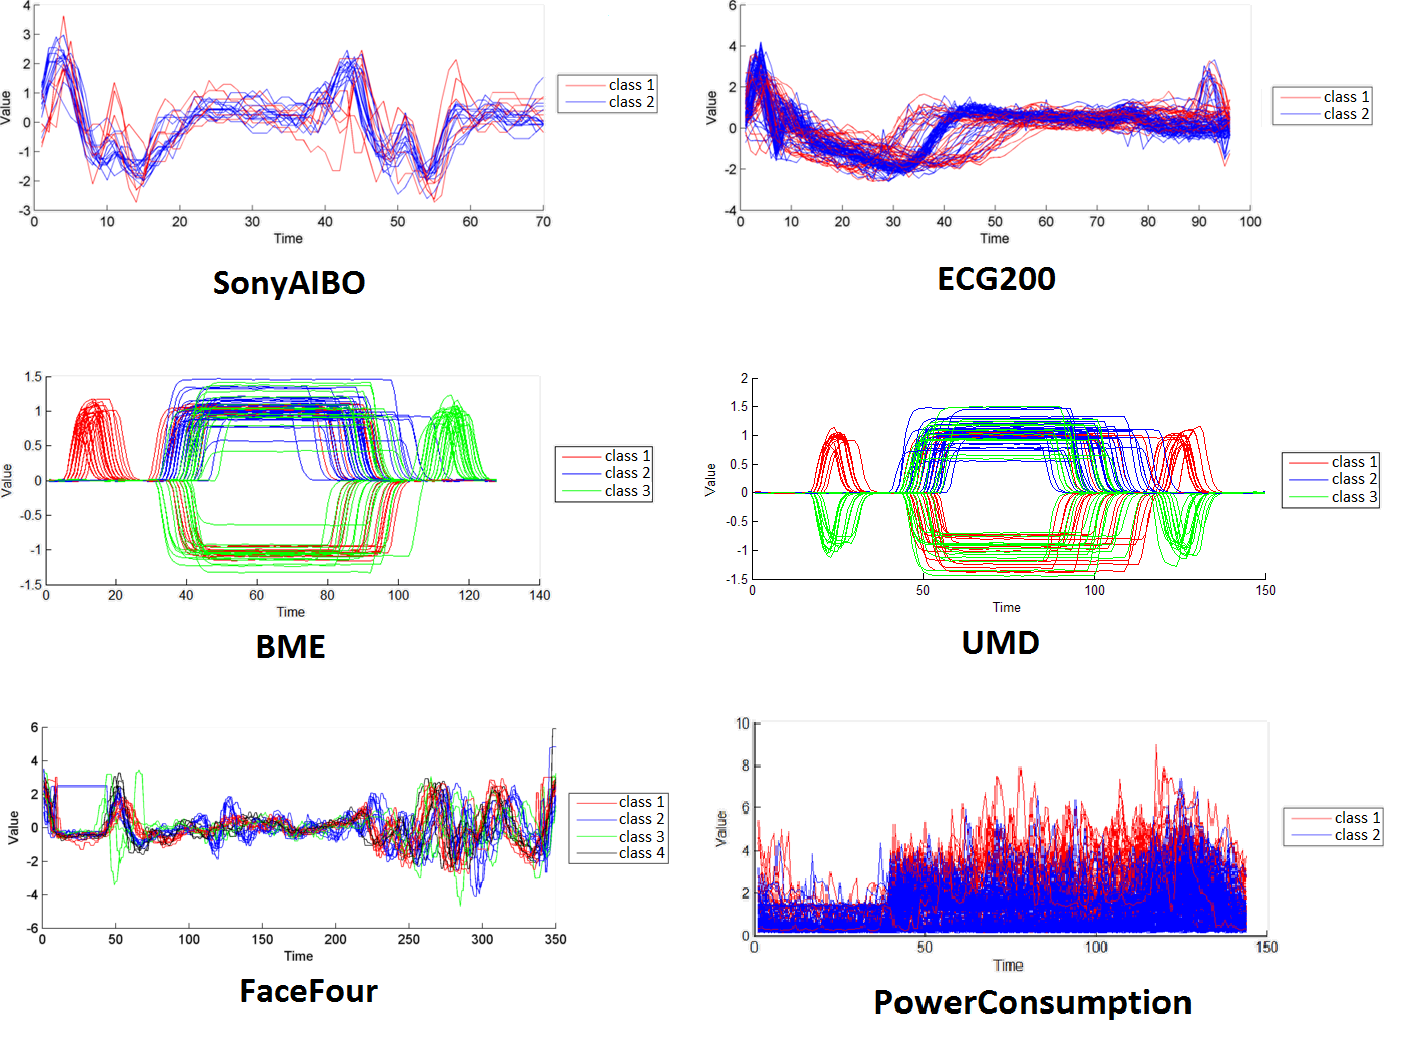
\includegraphics[width=0.95\linewidth]{images/dataset_exp}
	\caption{Temporal representation of some datasets (SonyAIBO, ECG200, BME, UMD, FaceFour, PowerConsumption) considered in the experiments.}
	\label{fig:dataset}
\end{figure}

\noindent The results of the learned metrics $D$ and $D_{\mathcal{H}}$ are compared to those of three \textit{a priori} combined metrics $D_{Lin}, D_{Geom}, D_{Sig}$ (Eqs. \ref{eq:DLin}, \ref{eq:DGeom}, \ref{eq:DSig}) and five alternative uni-modal metrics covering: 
\begin{enumerate}
	\item The standard  Euclidean distance $d_A$ (Eq. \ref{eq:A}) and Dynamic time warping\footnote{In this chapter, the term {\sc dtw} denotes the classically value-based metric computed after an alignment of the time series obtained with the {\sc dtw} algorithm with a value-based cost function.} {\sc dtw} (Eq. \ref{eq:DTW})
	\item The behavior-based measures  $d_B$ (Eq. \ref{eq:B}) and $d_{B-\mbox{\sc dtw}}$ its counterpart  for asynchronous time series, that is $d_B$ is evaluated once time series are synchronized using dynamic programing
	\item The frequential-based metric  $d_F$ (Eq. \ref{eq:F}). 
\end{enumerate}

\begin{table}[h!]
	\small
	\centering
	\renewcommand{\arraystretch}{0.85}
	\resizebox{1\textwidth}{!}{
		\setlength{\tabcolsep}{1pt}
		\begin{tabular}{llll}
			\hline
			Symbol & Name & Equation reference & Description \\
			\hline
			$d_A$ 				& Value-based dissimilarity			& Eq. \ref{eq:A} 				& Euclidean distance\\
			$d_B$ 				& Behavior-based dissimilarity 		& Eq. \ref{eq:B} 				& Behavior metric based on cort\\
			\textsc{dtw}		& Dynamic time warping 				& Eqs. \ref{eq:DTW} \& \ref{eq:A}& Euclidean distance after alignment\\
			$d_{B-\mbox{\sc dtw}}$ & Behavior-based aligned dissimilarity & Eqs. \ref{eq:DTW} \& \ref{eq:B}& Behavior metric based on cort after alignment\\
			$d_F$ 				& Frequential-based dissimilarity 	& Eq. \ref{eq:F} 				& Frequential  metric based on Fourier transform\\
			$D_{Lin}$ 			& Linear combined metric 			& Eq. \ref{eq:DLin} 			& Combines $d_A$ and $d_B$ (resp. \textsc{dtw} and $d_{B-\mbox{\sc dtw}}$) \\
			$D_{Geom}$ 			& Geometric combined metric 		& Eq. \ref{eq:DGeom} 			& Combines $d_A$ and $d_B$ (resp. \textsc{dtw} and $d_{B-\mbox{\sc dtw}}$) \\
			$D_{Sig}$ 			& Sigmoid combined metric 			& Eq. \ref{eq:DSig} 			& Combines $d_A$ and $d_B$ (resp. \textsc{dtw} and $d_{B-\mbox{\sc dtw}}$) \\
			$D$ 				& Linear learned metric 				& Eq. \ref{eq:dissimilarity_learn} 			 & \textsc{m$^2$tml} linear combined metric\\ 
			$D_{\mathcal{H}}$  	& Non-linear learned metric 			& Eq. \ref{eq:dissimilarity_learn_NonLinear} & \textsc{m$^2$tml} non-linear combined metric with a Gaussian kernel\\
			\hline
		\end{tabular}}
		\caption{Considered metric in the experiments}
		\label{tab:metric}
	\end{table}
	
\noindent Table \ref{tab:metric} recalls briefly the considered metrics in the experiments. The \textit{a priori} combined metrics ($D_{Lin}, D_{Geom}, D_{Sig}$) rely, on 2 log-normalized dissimilarities $d_{A}$, $d_{B}$ (resp. {\sc dtw}, $d_{B-\mbox{\sc dtw}}$ for asynchronous time series). The alternative metrics and the \textit{a priori} combined metrics are evaluated  as usual by involving all time series elements ({\it i.e.}, at the global scale). For $D$ and $D_{\mathcal{H}}$, we consider a 21-dimensional embedding space  $\mathcal{E}$ that relies, for synchronous (resp. asynchronous) data, on 3 log-normalized dissimilarities $d_{A}^{s}$, $d_{B}^{s}$ (resp. {\sc dtw}$^{s}$, $d_{B-\mbox{\sc dtw}}^{s}$), and $d_{F}^{s}$, at 7 temporal granularities $s \in \{0,...,6\}$ obtained by binary segmentation, described in Section \ref{sec:Pairwise_embedding}.

%-----------------------------------------------------------------------------
\section{Experimental protocol}
The different metrics can be split into two categories. For those without parameters to tune ($d_A$, \textsc{dtw}), the $1-$NN classifier is applied directly on the test set. For those that require to tune parameters ($d_B$, $d_{B-\mbox{\sc dtw}}$, $D_{Lin}$, $D_{Geom}$, $D_{Sig}$, $D$, $D_{\mathcal{H}}$), we recall briefly the grid search and cross-validation procedure (Section \ref{sec:model_selection}). When a learning algorithm requires to tune some parameters, to avoid overfitting, the training set can be divided into two sets: a learning and a validation set. The model is learnt for each combination of parameters (grid search) on the learning set and evaluated on the validation set. The model with the lowest error on the validation set is retained. An other alternative is cross-validation, which partitions the training set into $v$ folds, performs the learning on one subset, and validates on the $v-1$ other subsets. To take into account of variability within the data, multiple rounds of cross-validation are performed using different partitions, and the validation results are averaged over the rounds. Note that for unbalanced datasets in classification problems, it is recommended to use stratified sampling. Table \ref{tab:param} resumes the parameter ranges for each metric. We recall that the parameters retained are those that:
\begin{itemize}
	\item[-] \textbf{First}, minimize the average classification error on the validation set.
	\item[-] \textbf{Secondly}, in the case of multiple solutions leading to equal performances, the most discriminant one is retained (\textit{i.e.}, making closer pull pairs and far away push pairs). Precisely, it minimizes the ratio $\frac{d_{intra}}{d_{inter}}$ where $d_{intra}$ and $d_{inter}$ stands respectively to the mean of all intraclass and interclass distances.
\end{itemize} 
\noindent As $D$ and $D_{\mathcal{H}}$ involves several parameters to be tuned, we detail hereafter the procedure. The combined metrics $D$ and $D_{\mathcal{H}}$  ($\kappa$ as the Gaussian kernel) are learned respectively under $L_1$ and $L_2$ regularization, using \textsc{liblinear}  and \textsc{libsvm} libraries \cite{Fan2008,Hsu2008}. The parameters are estimated on a validation set by line/grid search. A cross-validation and stratified sampling for unbalanced datasets are used.  Particularly, for each  couple ($r$, $\lambda$) $r \in \{1, 4, 10\}$ and $\lambda \in \{0, 10, 30\}$, the pairwise {\sc svm} parameters ($C,\alpha, \gamma$) are learned by grid search as indicated in Table \ref{tab:param}. 

\begin{table}[h!]
	\small
	\centering
	\renewcommand{\arraystretch}{0.85}
	\resizebox{1\textwidth}{!}{
		\setlength{\tabcolsep}{1pt}
		\begin{tabular}{lccl}
			\hline
			Dissimilarity & Parameter & Ranges & Description\\
			\hline
			$d_{B}$, $d_{B-\mbox{\sc dtw}}$ & $r$       & $\{1, 2, 3, , \ldots, q-1\}$ 					& Order of behavior-based metric\\
			$D_{Lin}, D_{Geom}, D_{Sig}$ & $\beta$ & $\{0,0.1, \ldots, 1\}$ 					& Trade-off between value and behavior components\\
			$D$, $D_{\mathcal{H}}$  & $\lambda$ & $\{0, 10, 30\}$ 								& Strength of the '{\it push}' term \\
			$D$, $D_{\mathcal{H}}$  & $r$       & $\{1, 4, 10\}$ & Order of behavior-based metrics\\			
			$D$, $D_{\mathcal{H}}$  & $C$       & $\{10^{-3}, 0.5, 1, 5, 10, 20, 30, ..., 150\}$& Parameter of \textsc{svm}\\
			$D$, $D_{\mathcal{H}}$  & $\alpha$  & $\{1,2,3\}$     								& Size of the $m=\alpha.k$ neighborhood\\
			$D_{\mathcal{H}}$       & $\gamma$  & $\{10^{-3}, 10^{-2}, \ldots, 10^{3}\}$ 		& Parameter of the Gaussian kernel\\
			\hline
		\end{tabular}}
		\caption{Parameter ranges}
		\label{tab:param}
\end{table}
	
Note that the temporal order $r$ for the behavior-based metrics $d_B$ is noise-dependent, typically 1 is retained for noise-free data. The parameter $\lambda$ corresponds to the strength of the '{\it push}' term; precisely, if no, moderate or  strong '{\it push}'  is required during the training process, a $\lambda$ value of  0, 10 and 30 is learned, respectively. 
%-----------------------------------------------------------------------------
\newpage
\section{Results and discussion}
In this section, we first present a summary table of the quantitivative results obtained in the experiment. Secondly, we present an analysis of the performances of the different metrics. Finally, we present the ability of our proposed approach \textsc{m$^2$tml} to extract discriminative features.

\subsection{Results}
Table \ref{tab-resu} reports the 1-NN classification test errors based on uni-modal metrics  (first 5 columns), on three \textit{a priori} combined metrics ($D_{Lin}, D_{Geom}, D_{Sig}$) and on  $D$ and $D_{\mathcal{H}}$. The results for each dataset that are statistically and significantly better than the best performance are indicated in bold (Z-test at  5\% risk detailed in Section \ref{sec:ClassificationEvaluation}). The last column '{\sc warp}' indicates the synchronous (\checkmark) or asynchronous ($\times$) data type. \\ 
Data that need '{\sc warp}' are situated above the line. For each type of delay ('{\sc warp}' or non-'{\sc warp}'), the datasets are ordered from the less challenging datasets according to the performance of the classically used distances ($d_A$ or {\sc dtw}) to the most challenging datasets.

\begin{table}[h!]
	\small
	\centering
	\renewcommand{\arraystretch}{0.8}
	\resizebox{1\textwidth}{!}{
		\setlength{\tabcolsep}{1pt}
		\begin{tabular}{|l|ccccc|ccc|ccc|}
			\hline
			& \multicolumn{5}{c|}{Alternative uni-modal metrics} & \multicolumn{3}{c|}{A priori combinations} & \multicolumn{2}{c}{{\sc m}$^2${\sc tml}} & {\sc warp}  \\
			\cline{2-12} 
			Dataset & $d_A$ & $d_B$ & $d_F$ & $\mbox{\sc dtw}$ & $d_{B-\mbox{\sc dtw}}$ & $D_{Lin}$ & $D_{Geom}$ & $D_{Sig}$ & $D (\lambda^*)$ & $D_{\mathcal{H}} (\lambda^*)$ & {\sc warp}  \\
			\hline
			1 ItalyPowerD     	& 0.045 & \textbf{0.028}& 0.078 & 0.050 & 0.055    & \textbf{0.028} & \textbf{0.028} & \textbf{0.030} & \textbf{0.034} (0) & 0.046 (0) & $\times$  \\
			2 CinCECGtorso        & 0.103 & 0.367 & 0.167 & 0.349 & 0.367  & \textbf{0.094} & \textbf{0.094} & \textbf{0.093} & \textbf{0.092} (0)  & \textbf{0.088} (0) & $\times$   \\	
			3 BME      & 0.173 & 0.160 & 0.373 & 0.107 & 0.120 & 0.107 & 0.107 & 0.107 & \textbf{0.007} (0) & \textbf{0.007} (0) 	     & $\times$ \\									
			4 ECG200              & \textbf{0.120} & \textbf{0.070}& 0.160 & 0.230& 0.190    & \textbf{0.070} & \textbf{0.070} & \textbf{0.070} & \textbf{0.080} (0)  & \textbf{0.080} (0) & $\times$  \\
			5 SonyAIBOII          & \textbf{0.141} & \textbf{0.142} & \textbf{0.128} & 0.169 & 0.194     & \textbf{0.142} & \textbf{0.142} & \textbf{0.144} & \textbf{0.162} (0)  & \textbf{0.142} (0) & $\times$  \\			
			6 Coffee              & 0.250 & \textbf{0.000}    & 0.357 & 0.179 & 0.143     & \textbf{0.000} & \textbf{0.000} & \textbf{0.071} & 0.143 (0)     & \textbf{0.036} (10) &$\times$  \\						
			7 ECG5Days            & 0.203 & 0.153 & \textbf{0.006} & 0.232 & 0.236    & 0.203 & 0.203 & 0.203 & \textbf{0.012} (10) & 0.024 (0)  & $\times$   \\
			8 SonyAIBO            & 0.305 & 0.308 & 0.258 & 0.275 & 0.343     & 0.308 & 0.308 & 0.293 & \textbf{0.188} (0)  & \textbf{0.228} (0) & $\times$   \\							
			9 Adiac               & 0.389 & \textbf{0.297} & \textbf{0.261} & 0.396 & 0.338     & 0.373 & 0.363 & 0.402 & 0.358 (0)  & 0.361 (0) & $\times$\\
			10 Beef                & 0.467 & 0.300 & 0.500 & 0.500 & 0.500     & 0.367 & 0.267 & 0.467 & \textbf{0.033} (0) & 0.257 (0) & $\times$   \\	
			\hline		
			11 Trace               & 0.240 & 0.240 & 0.140 & \textbf{0.000}    & \textbf{0.000}        & \textbf{0.000} & \textbf{0.000} & \textbf{0.000} & \textbf{0.000} (0)    & \textbf{0.010} (0)  & \checkmark \\	
			12 CBF                 & 0.148 & 0.140 & 0.382 & \textbf{0.003} & \textbf{0.000}        & \textbf{0.000} & \textbf{0.000} & \textbf{0.000} & 0.097 (0) & \textbf{0.008} (0)  & \checkmark \\										
			13 CC                  & 0.120 & 0.113 & 0.383 & \textbf{0.007} & 0.027     & \textbf{0.007} & \textbf{0.007} & \textbf{0.007} &\textbf{0.007} (0) & \textbf{0.007} (0) & \checkmark \\		
			14 DiatomSizeR     	& 0.065 & 0.076 & 0.069 & \textbf{0.033} & \textbf{0.029}     & \textbf{0.033} & \textbf{0.033} & \textbf{0.042} & 0.088 (0)  & \textbf{0.029} (0) & \checkmark \\			
			15 Symbols             & 0.101 & 0.111 & 0.080 & \textbf{0.050} & \textbf{0.043}     & \textbf{0.051} & \textbf{0.050} & \textbf{0.052} & 0.102 (10) & \textbf{0.057} (0) & \checkmark \\
			16 GunPoint            & 0.087 & 0.113 & \textbf{0.027} & 0.093 & \textbf{0.027}     & \textbf{0.027} & \textbf{0.027} & \textbf{0.040} & \textbf{0.033} (0) & \textbf{0.053} (10) & \checkmark \\
			17 FacesUCR            & 0.231 & 0.227 & 0.175 & 0.095 & 0.102     & 0.098 & 0.098 & 0.099 & \textbf{0.068}  (10) & \textbf{0.068} (0) & \checkmark \\
			18 TwoLeadECG          & 0.253 & 0.153 & 0.103 & 0.096 & \textbf{0.008}   & \textbf{0.005} & \textbf{0.005} & 0.018 & \textbf{0.006} (0)  & 0.016 (10) & \checkmark \\	
			19 UMD 		& 0.194 & 0.222 & 0.229 & 0.118 & \textbf{0.090} & 0.111 & 0.111 & 0.118 & 0.104  (0) & \textbf{0.042} (0) & \checkmark \\ 			
			20 MoteStrain          & \textbf{0.121} & 0.263& 0.278 & 0.165& 0.171     & 0.260 & 0.248 & 0.188 & 0.185 (0)  & 0.179 (0) & \checkmark \\						
			21 Lighting2           & \textbf{0.246} & \textbf{0.246} & \textbf{0.148} & \textbf{0.131} & \textbf{0.213} & \textbf{0.131} & \textbf{0.131} & \textbf{0.131} & \textbf{0.213} (0)  & \textbf{0.131} (0) & \checkmark \\
			22 OliveOil            & \textbf{0.133} & \textbf{0.133} & \textbf{0.167} & \textbf{0.200} & \textbf{0.100}    & \textbf{0.133} & \textbf{0.133} & \textbf{0.133} & \textbf{0.167} (0)  & \textbf{0.100} (10) & \checkmark \\			
			23 FISH                & 0.217 & \textbf{0.149} & 0.229 & \textbf{0.166} & \textbf{0.137}   & \textbf{0.109} & \textbf{0.137} & \textbf{0.126} & \textbf{0.149} (0)  & 0.240 (0) & \checkmark  \\			
			24 FaceFour            & 0.216 & 0.216 & 0.239 & 0.170 & 0.136 & 0.170 & 0.170 & 0.170 & \textbf{0.023} (0)     & 0.114 (0)  & \checkmark \\
			25 SwedishLeaf         & 0.211 & 0.186 & 0.146 & 0.208 & \textbf{0.109} & \textbf{0.115} & \textbf{0.110} & \textbf{0.125} & \textbf{0.142} (0) & \textbf{0.114} (0) & \checkmark \\			
			26 MedicalImages       & 0.316 & 0.313 & 0.345 & \textbf{0.263} & 0.290     & \textbf{0.263} & \textbf{0.263} & \textbf{0.263} & \textbf{0.237} (0) & \textbf{0.241} (10) & \checkmark \\
			27 Lighting7           & \textbf{0.425} & \textbf{0.411} & \textbf{0.316} & \textbf{0.274} & \textbf{0.288}     & \textbf{0.342} & \textbf{0.356} & \textbf{0.342} & \textbf{0.411} (0)  & \textbf{0.233} (0) & \checkmark \\
			28 PowerCons           & \textbf{0.366} & 0.445 & \textbf{0.315} & 0.397 & 0.401     & 0.401 & 0.401 & 0.401 & \textbf{0.318} (0)  & \textbf{0.342} (0) & \checkmark \\												
			29 OSULeaf             & 0.484 & 0.475 & 0.426 & 0.409 & \textbf{0.265}    & \textbf{0.264} & \textbf{0.264} & \textbf{0.322} & 0.421 (0)  & 0.388 (0)  & \checkmark \\
			30 InlineSkate         & \textbf{0.658} & \textbf{0.658} & 0.675 & \textbf{0.616} & \textbf{0.623}     & \textbf{0.605} & \textbf{0.605} & \textbf{0.602} & 0.833  (10) & \textbf{0.625} (0) & \checkmark \\
			\hline
		\end{tabular}
	}
	\caption{1-NN test error rates for standard, \textit{a priori} combined and {\sc m}$^2${\sc tml} measures.}
	\label{tab-resu}
\end{table}
%\vspace{-1cm}

% dA, DTW, D, DH
%\begin{table}[h!] \small \centering \renewcommand{\arraystretch}{0.8} \resizebox{1\textwidth}{!}{ \setlength{\tabcolsep}{1pt} \begin{tabular}{|l|cccc|} \hline 
%			Dataset	& $d_A$	& $DTW$	& $D$	& $D_H$ \\ 
%			\hline
%			ItalyPowerDemand	& \textbf{0.045}	&0.050	& \textbf{0.034}	& \textbf{0.046}\\ 
%			CinCECGtorso	& \textbf{0.103}	&0.349	& \textbf{0.092}	& \textbf{0.088}\\ 
%			BME	&0.173	&0.107	& \textbf{0.007}	& \textbf{0.007}\\ 
%			ECG200	& \textbf{0.120}	&0.230	& \textbf{0.080}	& \textbf{0.080}\\ 
%			SonyAIBORobotSurfaceII	& \textbf{0.141}	&0.169	& \textbf{0.162}	& \textbf{0.142}\\ 
%			Coffee	&0.250	&0.179	& \textbf{0.143}	& \textbf{0.036}\\ 
%			ECGFiveDays	&0.203	&0.232	& \textbf{0.012}	&0.024\\ 
%			SonyAIBORobotSurface	&0.305	&0.275	& \textbf{0.188}	&0.228\\ 
%			Adiac	& \textbf{0.389}	& \textbf{0.396}	& \textbf{0.358}	& \textbf{0.361}\\ 
%			Beef	&0.467	&0.500	& \textbf{0.033}	&0.257\\ 
%			Trace	&0.240	& \textbf{0.000}	& \textbf{0.000}	& \textbf{0.010}\\ 
%			CBF	&0.148	& \textbf{0.003}	&0.097	& \textbf{0.008}\\ 
%			syntheticcontrol	&0.120	& \textbf{0.007}	& \textbf{0.007}	& \textbf{0.007}\\ 
%			DiatomSizeReduction	&0.065	& \textbf{0.033}	&0.088	& \textbf{0.029}\\ 
%			Symbols	&0.101	& \textbf{0.050}	&0.102	& \textbf{0.057}\\ 
%			GunPoint	&0.087	&0.093	& \textbf{0.033}	& \textbf{0.053}\\ 
%			FacesUCR	&0.231	&0.095	& \textbf{0.068}	& \textbf{0.068}\\ 
%			TwoLeadECG	&0.253	&0.096	& \textbf{0.006}	&0.016\\ 
%			UMD	&0.194	&0.118	& \textbf{0.104}	& \textbf{0.042}\\ 
%			MoteStrain	& \textbf{0.121}	&0.165	&0.185	&0.179\\ 
%			Lighting2	& \textbf{0.246}	& \textbf{0.131}	& \textbf{0.213}	& \textbf{0.131}\\ 
%			OliveOil	& \textbf{0.133}	& \textbf{0.200}	& \textbf{0.167}	& \textbf{0.100}\\ 
%			FISH	&0.217	& \textbf{0.166}	& \textbf{0.149}	&0.240\\ 
%			FaceFour	&0.216	&0.170	& \textbf{0.023}	&0.114\\ 
%			SwedishLeaf	&0.211	&0.208	& \textbf{0.142}	& \textbf{0.114}\\ 
%			MedicalImages	&0.316	& \textbf{0.263}	& \textbf{0.237}	& \textbf{0.241}\\ 
%			Lighting7	&0.425	& \textbf{0.274}	&0.411	& \textbf{0.233}\\ 
%			PowerConsumption	& \textbf{0.366}	&0.397	& \textbf{0.318}	& \textbf{0.342}\\ 
%			OSULeaf	&0.484	& \textbf{0.409}	& \textbf{0.421}	& \textbf{0.388}\\ 
%			InlineSkate	& \textbf{0.658}	& \textbf{0.616}	&0.833	& \textbf{0.625}\\ 
%			\hline \end{tabular} } \caption{ Error with Z-test at confidence 10\% } \label{tab-resu} \end{table} 


%% DLin DGeom DSig D and D-H
%\begin{table}[h!] \small \centering \renewcommand{\arraystretch}{0.8} \resizebox{1\textwidth}{!}{ \setlength{\tabcolsep}{1pt} \begin{tabular}{|l|ccccc|} \hline 
%			Dataset	& $Dlin$	& $Dgeom$	& $Dsig$	& $D$	& $D-H$ \\ 
%			\hline
%			ItalyPowerDemand	& \textbf{0.028}	& \textbf{0.028}	& \textbf{0.030}	& \textbf{0.034}	&0.046\\ 
%			CinCECGtorso	& \textbf{0.094}	& \textbf{0.094}	& \textbf{0.093}	& \textbf{0.092}	& \textbf{0.088}\\ 
%			BME	&0.107	&0.107	&0.107	& \textbf{0.007}	& \textbf{0.007}\\ 
%			ECG200	& \textbf{0.070}	& \textbf{0.070}	& \textbf{0.070}	& \textbf{0.080}	& \textbf{0.080}\\ 
%			SonyAIBORobotSurfaceII	& \textbf{0.142}	& \textbf{0.142}	& \textbf{0.144}	& \textbf{0.162}	& \textbf{0.142}\\ 
%			Coffee	& \textbf{0.000}	& \textbf{0.000}	& \textbf{0.071}	&0.143	& \textbf{0.036}\\ 
%			ECGFiveDays	&0.203	&0.203	&0.203	& \textbf{0.012}	&0.024\\ 
%			SonyAIBORobotSurface	&0.308	&0.308	&0.293	& \textbf{0.188}	&0.228\\ 
%			Adiac	& \textbf{0.373}	& \textbf{0.363}	& \textbf{0.402}	& \textbf{0.358}	& \textbf{0.361}\\ 
%			Beef	&0.367	&0.267	&0.467	& \textbf{0.033}	&0.257\\ 
%			Trace	& \textbf{0.000}	& \textbf{0.000}	& \textbf{0.000}	& \textbf{0.000}	& \textbf{0.010}\\ 
%			CBF	& \textbf{0.000}	& \textbf{0.000}	& \textbf{0.000}	&0.097	&0.008\\ 
%			syntheticcontrol	& \textbf{0.007}	& \textbf{0.007}	& \textbf{0.007}	& \textbf{0.007}	& \textbf{0.007}\\ 
%			DiatomSizeReduction	& \textbf{0.033}	& \textbf{0.033}	& \textbf{0.042}	&0.088	& \textbf{0.029}\\ 
%			Symbols	& \textbf{0.051}	& \textbf{0.050}	& \textbf{0.052}	&0.102	& \textbf{0.057}\\ 
%			GunPoint	& \textbf{0.027}	& \textbf{0.027}	& \textbf{0.040}	& \textbf{0.033}	& \textbf{0.053}\\ 
%			FacesUCR	&0.098	&0.098	&0.099	& \textbf{0.068}	& \textbf{0.068}\\ 
%			TwoLeadECG	& \textbf{0.005}	& \textbf{0.005}	&0.018	& \textbf{0.006}	&0.016\\ 
%			UMD	&0.111	&0.111	&0.118	& \textbf{0.104}	& \textbf{0.042}\\ 
%			MoteStrain	&0.260	&0.248	& \textbf{0.188}	& \textbf{0.185}	& \textbf{0.179}\\ 
%			Lighting2	& \textbf{0.131}	& \textbf{0.131}	& \textbf{0.131}	& \textbf{0.213}	& \textbf{0.131}\\ 
%			OliveOil	& \textbf{0.133}	& \textbf{0.133}	& \textbf{0.133}	& \textbf{0.167}	& \textbf{0.100}\\ 
%			FISH	& \textbf{0.109}	& \textbf{0.137}	& \textbf{0.126}	& \textbf{0.149}	&0.240\\ 
%			FaceFour	&0.170	&0.170	&0.170	& \textbf{0.023}	&0.114\\ 
%			SwedishLeaf	& \textbf{0.115}	& \textbf{0.110}	& \textbf{0.125}	&0.142	& \textbf{0.114}\\ 
%			MedicalImages	& \textbf{0.263}	& \textbf{0.263}	& \textbf{0.263}	& \textbf{0.237}	& \textbf{0.241}\\ 
%			Lighting7	& \textbf{0.342}	& \textbf{0.356}	& \textbf{0.342}	&0.411	& \textbf{0.233}\\ 
%			PowerConsumption	&0.401	&0.401	&0.401	& \textbf{0.318}	& \textbf{0.342}\\ 
%			OSULeaf	& \textbf{0.264}	& \textbf{0.264}	& \textbf{0.322}	&0.421	&0.388\\ 
%			InlineSkate	& \textbf{0.605}	& \textbf{0.605}	& \textbf{0.600}	&0.833	& \textbf{0.625}\\ 
%			\hline \end{tabular} } \caption{ Error with Z-test at confidence 10\% } \label{tab-resu} \end{table} 

%% Unimodal and D et DH
%\begin{table}[h!] \small \centering \renewcommand{\arraystretch}{0.8} \resizebox{1\textwidth}{!}{ \setlength{\tabcolsep}{1pt} \begin{tabular}{|l|ccccccc|} \hline 
%			Dataset	& $DE$	& $corT$	& $DFFT$	& $DTW$	& $DTWcorT$	& $D$	& $D-H$ \\ 
%			\hline
%			ItalyPowerDemand	&0.045	& \textbf{0.028}	&0.078	&0.050	&0.055	& \textbf{0.034}	&0.046\\ 
%			CinCECGtorso	& \textbf{0.103}	&0.367	&0.167	&0.349	&0.367	& \textbf{0.092}	& \textbf{0.088}\\ 
%			BME	&0.173	&0.160	&0.373	&0.107	&0.120	& \textbf{0.007}	& \textbf{0.007}\\ 
%			ECG200	& \textbf{0.120}	& \textbf{0.070}	&0.160	&0.230	&0.190	& \textbf{0.080}	& \textbf{0.080}\\ 
%			SonyAIBORobotSurfaceII	& \textbf{0.141}	& \textbf{0.142}	& \textbf{0.128}	&0.169	&0.194	&0.162	& \textbf{0.142}\\ 
%			Coffee	&0.250	& \textbf{0.000}	&0.357	&0.179	&0.143	&0.143	& \textbf{0.036}\\ 
%			ECGFiveDays	&0.203	&0.153	& \textbf{0.006}	&0.232	&0.236	& \textbf{0.012}	&0.024\\ 
%			SonyAIBORobotSurface	&0.305	&0.308	&0.258	&0.275	&0.343	& \textbf{0.188}	&0.228\\ 
%			Adiac	&0.389	& \textbf{0.297}	& \textbf{0.261}	&0.396	&0.338	&0.358	&0.361\\ 
%			Beef	&0.467	&0.300	&0.500	&0.500	&0.500	& \textbf{0.033}	&0.257\\ 
%			Trace	&0.240	&0.240	&0.140	& \textbf{0.000}	& \textbf{0.000}	& \textbf{0.000}	& \textbf{0.010}\\ 
%			CBF	&0.148	&0.140	&0.382	&0.003	& \textbf{0.000}	&0.097	&0.008\\ 
%			syntheticcontrol	&0.120	&0.113	&0.383	& \textbf{0.007}	&0.027	& \textbf{0.007}	& \textbf{0.007}\\ 
%			DiatomSizeReduction	&0.065	&0.076	&0.069	& \textbf{0.033}	& \textbf{0.029}	&0.088	& \textbf{0.029}\\ 
%			Symbols	&0.101	&0.111	&0.080	& \textbf{0.050}	& \textbf{0.043}	&0.102	& \textbf{0.057}\\ 
%			GunPoint	&0.087	&0.113	& \textbf{0.027}	&0.093	& \textbf{0.027}	& \textbf{0.033}	& \textbf{0.053}\\ 
%			FacesUCR	&0.231	&0.227	&0.175	&0.095	&0.102	& \textbf{0.068}	& \textbf{0.068}\\ 
%			TwoLeadECG	&0.253	&0.153	&0.103	&0.096	& \textbf{0.008}	& \textbf{0.006}	&0.016\\ 
%			UMD	&0.194	&0.222	&0.229	&0.118	& \textbf{0.090}	& \textbf{0.104}	& \textbf{0.042}\\ 
%			MoteStrain	& \textbf{0.121}	&0.263	&0.278	&0.165	&0.171	&0.185	&0.179\\ 
%			Lighting2	& \textbf{0.246}	& \textbf{0.246}	& \textbf{0.148}	& \textbf{0.131}	& \textbf{0.213}	& \textbf{0.213}	& \textbf{0.131}\\ 
%			OliveOil	& \textbf{0.133}	& \textbf{0.133}	& \textbf{0.167}	& \textbf{0.200}	& \textbf{0.100}	& \textbf{0.167}	& \textbf{0.100}\\ 
%			FISH	&0.217	& \textbf{0.149}	&0.229	& \textbf{0.166}	& \textbf{0.137}	& \textbf{0.149}	&0.240\\ 
%			FaceFour	&0.216	&0.216	&0.239	&0.170	&0.136	& \textbf{0.023}	&0.114\\ 
%			SwedishLeaf	&0.211	&0.186	&0.146	&0.208	& \textbf{0.109}	&0.142	& \textbf{0.114}\\ 
%			MedicalImages	&0.316	&0.313	&0.345	& \textbf{0.263}	&0.290	& \textbf{0.237}	& \textbf{0.241}\\ 
%			Lighting7	&0.425	&0.411	& \textbf{0.316}	& \textbf{0.274}	& \textbf{0.288}	&0.411	& \textbf{0.233}\\ 
%			PowerConsumption	& \textbf{0.366}	&0.445	& \textbf{0.315}	&0.397	&0.401	& \textbf{0.318}	& \textbf{0.342}\\ 
%			OSULeaf	&0.484	&0.475	&0.426	&0.409	& \textbf{0.265}	&0.421	&0.388\\ 
%			InlineSkate	& \textbf{0.658}	& \textbf{0.658}	&0.675	& \textbf{0.616}	& \textbf{0.623}	&0.833	& \textbf{0.625}\\ 
%			\hline \end{tabular} } \caption{ Error with Z-test at confidence 10\% } \label{tab-resu} \end{table} 



%-----------------------------------------------------------------------------
\newpage
%\section{Discussion}
\subsection{Comparison of the classification performances on the test set}
From Table \ref{tab-resu}, we can see first that the 1-NN classification reaches  the best results in: 
\begin{enumerate}
	\item Less than one-third of the data when based on unimodal metrics $d_A$, $d_B$ or $d_F$
	\item Slightly more than one-third for unimodal metrics $\mbox{\sc dtw}$ and $d_{B-\mbox{\sc dtw}}$ 
	\item Two-thirds (19 - 20 times on 30) when based on \textit{a priori} combined metrics $D_{Lin}$, $D_{Geom}$ and $D_{Sig}$
	\item More than two-thirds (21 times on 30)  when based on learned metrics $D$ or  $D_{\mathcal{H}}$.
\end{enumerate}
% i) less than one-third of the data when based on $d_A$, $d_B$ or $d_F$, ii) slightly more than one-third for  $\mbox{\sc dtw}$ and $d_{B-\mbox{\sc dtw}}$ and iii) more than two-thirds (23 times on 30)  when based on  $D$ or  $D_{\mathcal{H}}$.
Particularly, note that for nearly all datasets for which an uni-modal metric succeeds,  the {\sc m}$^2${\sc tml} metrics succeed similarly or lead to equivalent results.  
However, for  several challenging datasets ({\it e.g.} FaceFour, Beef, FaceUCR, SonyAIBO, BME, CinCECGTorso), {\sc m}$^2${\sc tml} realizes drastic improvements, to the best of our knowledge never achieved before  for these challenging public data. For instance, a score of 3\% is obtained for Beef against an error rate  varying from 30\% to 50\% for alternative metrics, and of 2.3\% obtained for FaceFour  v.s. 13\% to 23\% for alternative metrics.  Finally, $D$ and $D_{\mathcal{H}}$ are most datasets, either equivalent or better if only compared to the standard metrics $d_A$ (the Euclidean distance) and {\sc dtw}. 

\noindent If we compare the \textit{a priori} combined metrics ($D_{Lin}$, $D_{Geom}$, $D_{Sig}$) based on only the unimodal metrics involved in the combination (either $d_A$ and $d_B$ or $\mbox{\sc dtw}$ and $d_{B-\mbox{\sc dtw}}$), we observe that \textit{a priori} combined metrics achieved on two-third of the data with an equivalent or better score. Compared to the learned metrics ($D$, $D_{\mathcal{H}}$), the results are globally similar except for 8 datasets where the learned metrics perform better (FaceFour, Beef, ECG5Days, FaceUCR, SonyAIBO, PowerCons, BME, UMD) and one where the \textit{a priori} combined metrics perform better (OSULeaf). Note that the combined metric $D_{Sig}$ is limited to two components and can't be easily extend to other metrics in its combination. $D_{Lin}$ and $D_{Geom}$ could be easily extended and a proposition could be:
\begin{align}
	D_{Lin}(\textbf{x}_i,\textbf{x}_j) = \sum\limits_{h=1}^{p} \alpha_h d_h(\textbf{x}_i,\textbf{x}_j) \\
	D_{Geom}(\textbf{x}_i,\textbf{x}_j) = \prod\limits_{h=1}^{p} \alpha_h d_h(\textbf{x}_i,\textbf{x}_j)
\end{align}
However, by considering $p$ metrics $d_h$ the resulting models requires to optimize $p$ parameters. The grid search to find the best parameters $\alpha_h$ can become time consuming. The \textsc{m$^2$tml} approach has been proposed to prevent such an exhaustive grid search. \\
%\begin{itemize}
%	\item a priori vs unimodal : juste en prenant en compte les unimodales associées (dA,dB) les métriques combinées atteignent des scores équivalents ou meilleurs (CincECGTorso) sur les 2/3 des bases.
%	\item a priori vs learnt metric : on observe que les métriques apprises atteignent des scores similaires aux métriques a priori sauf sur certaines bases où la métrique apprise est meilleure (FaceFour, Beef, ECG5Days, FaceUCR, SonyAIBO, PowerCons, BME, UMD) et une seule où la métrique combinée a priori est meilleure (OSULeaf).
%	\item l'inconvénient de la métrique a priori est qu'elle ne permet de combiner que 2 modalités au niveau global. Dans le cadre de la métrique linéaire et exponentielle, on pourrait facilement étendre en ajoutant des métriques. Par exemple : $D_Lin = \sum\limits_{h=1}^{p} \alpha_h d_h$. L'inconvénient est qu'il y aurait autant de paramètres à optimiser qu'il y aurait de métriques 
%\end{itemize}

In the second part,  we perform a graphical analysis for a global comparison on the whole datasets.  In Fig. \ref{fig:error2}-a,  each dataset is projected according to, on the x-axis its best error rate obtained for $D$ and  $D_{\mathcal{H}}$, and on y-axis  its best performance \textit{w.r.t}  the standard amplitude-based metrics $d_A$  and  {\sc dtw}. 
In Fig. \ref{fig:error2}-b, the y-axis is related to the best error rate of the behavior-based metrics $d_B$  and  and $d_{B-\mbox{\sc dtw}}$.
In Fig. \ref{fig:error2}-c,  the y-axis is related to the best error rate of the two "non-warp" uni-modal metrics $d_A$ and $d_{B}$, .
In Fig. \ref{fig:error2}-d,  the y-axis is related to the best error rate of the two "warp" uni-modal metrics {\sc dtw} and $d_{B-\mbox{\sc dtw}}$ that are also the two most performant uni-modal metrics.
In Fig. \ref{fig:error2}-e,  the y-axis is related to the error rate of the frequential-based metric $d_F$. 
In Fig. \ref{fig:error2}-f,  the y-axis is related to the best error rate of the a priori-combined metrics $D_{Lin}, D_{Geom}, D_{Sig}$. \\
For all plots, let first give some interpretations. If the datasets are situated on the first bisector, it means that the considered metrics in x-axis and y-axis have equal performance. For datasets situated above the first bisector, it means in this case that {\sc m$^2$tml} method is better that the considered metrics in y-axis. Similarly, for datasets situated below the first bisector, it means in this case that the considered metrics in y-axis are better than {\sc m$^2$tml}. Less challenging datasets (low classification error rate) are situated near the origin and challenging dataset (high classification error rate) are situated far from the origin. \\
For all plots, we can note that the datasets are principally  projected above the first bisector, indicating higher error rates mostly obtained for uni-modal and \textit{a priori} combined metrics than for {\sc m}$^2${\sc tml}. For the less challenging datasets (near the origin of each graph), although almost projected near the bisector denoting equal performances for the compared metrics, {\sc m}$^2${\sc tml}  still  bring improvements with projections clearly positioned  above the bisector. Finally, from all plots, note that some datasets (Adiac, OSULeaf, InlineSkate) remains challenging for all studied metrics.

\begin{figure}[h!]
	\centering
	\subfloat[]{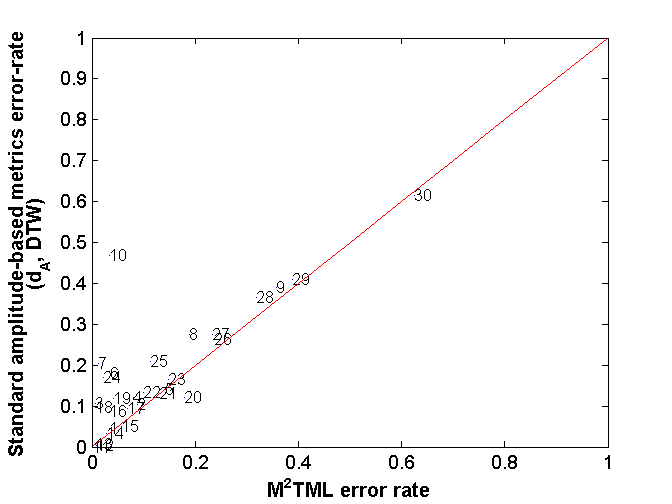
\includegraphics[width = 3in]{Stand_m2tml_2}}
	\subfloat[]{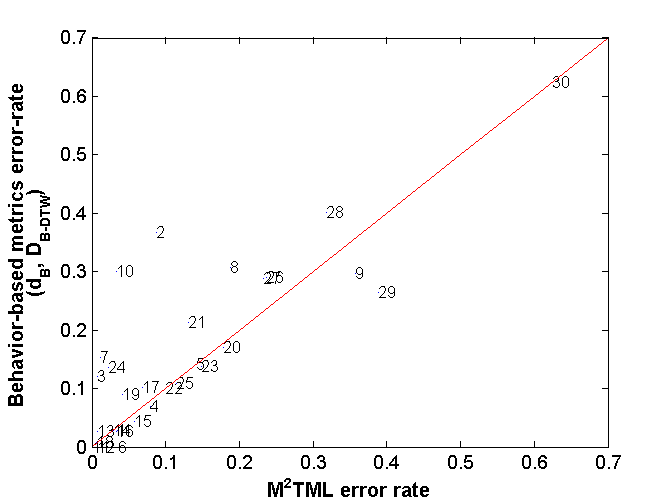
\includegraphics[width = 3in]{behavior_m2tml_2}}\
	\subfloat[]{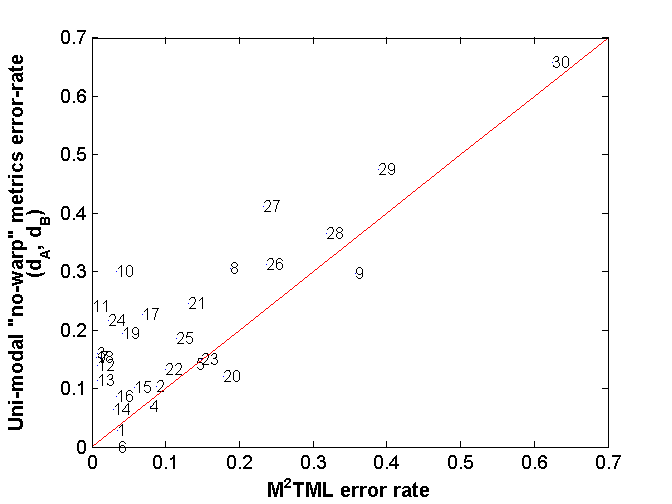
\includegraphics[width = 3in]{no_warp_m2tml_2}}
	\subfloat[]{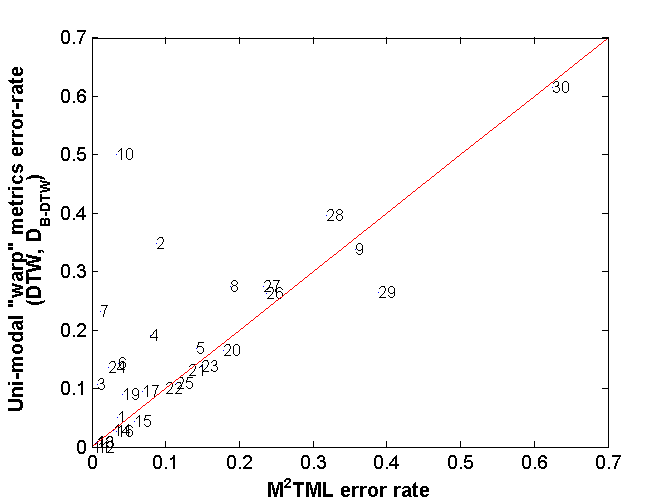
\includegraphics[width = 3in]{Unimod_m2tml_2}} \
	\subfloat[]{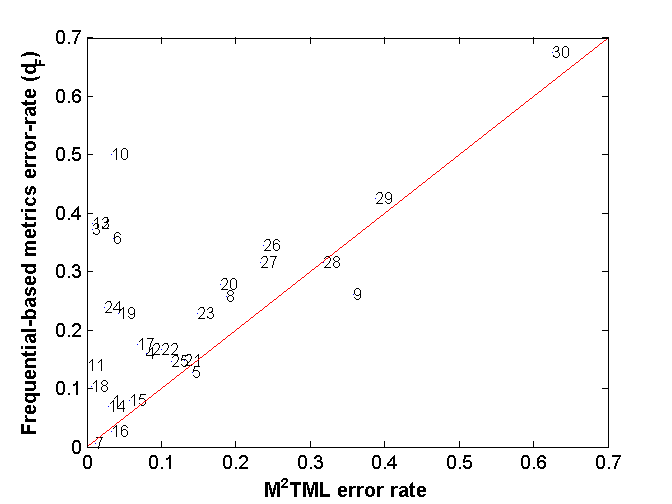
\includegraphics[width = 3in]{freq_m2tml_2}} 	\subfloat[]{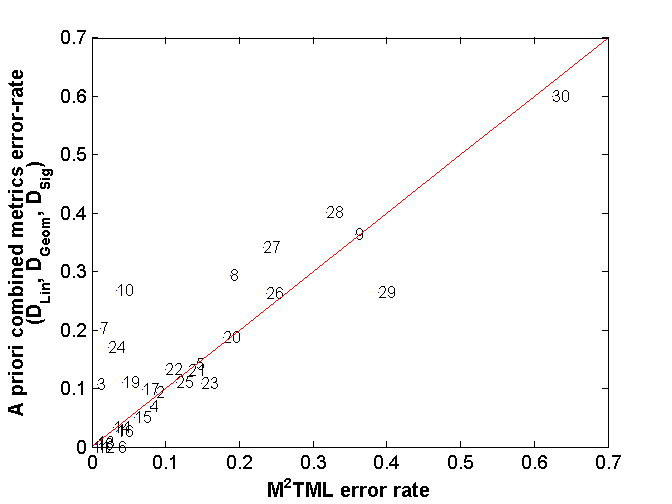
\includegraphics[width = 3in]{apriori_m2tml_2}}\	   
	\caption{(a) Standard amplitude-based (Euclidean distance $d_A$  and {\sc dtw}) vs. {\sc m}$^2${\sc tml} ($D$ and $D_{\mathcal{H}}$) metrics. 
	(b) Behavior-based ($d_B$  and $d_{B-\mbox{\sc dtw}}$) vs. {\sc m}$^2${\sc tml} metrics. 	
	(c) No-warp ($d_A$  and $d_{B}$) vs. {\sc m}$^2${\sc tml} metrics. 
	(d) Warp ({\sc dtw}  and $d_{B-\mbox{\sc dtw}}$) vs. {\sc m}$^2${\sc tml}  metrics. 	
	(e) Frequential-based ($d_F$) vs. {\sc m}$^2${\sc tml} metrics.
	(f) \textit{A priori} ($D_{Lin}$, $D_{Geom}$, $D_{Sig}$) vs. {\sc m}$^2${\sc tml} metrics. 
	}
	\label{fig:error2}
\end{figure}


\subsection{Analysis of the discriminative features}
For the learned metric $D$, thanks to the $L_1$ regularization, the learned {\sc svm} reveals the features that most differentiate pull from push pairs. We recall that the weight for each feature can be analyzed through the weight vector $\textbf{w}$ obtained by learning the {\sc svm} classifier. Table \ref{tab-feature} shows the sparse, muti-modal and multi-scale potential of {\sc m}$^2${\sc tml} approach.  It gives for each dataset, the weights of the top five 'discriminative' features that contribute to the definition of $D$.  For instance,   for FaceFour $D$ reaches an error of 2.3\% by combining, in the order of importance, the behavior $d_{B-\mbox{\sc dtw}}$,  frequential $d_F$ and amplitude {\sc dtw} modalities, at the global ($I^0$) and  local ($I^4$, $I^5$, $I^2$) scales. For Beef, the learned model is very sparse as $D$ involves only the behavior modality based on the segment $I^3$ ($d_B^3$). Note that if we look at only the most discriminative feature (1st column), the {\sc m}$^2${\sc tml} method helps to localize discriminative modality and a specific temporal scale (localization) that could not be easily guessed \textit{a priori} (\textit{e.g.}, Lightning7: behavior modality on the segment $I_6$ ($d_{B-\mbox{\sc dtw}}^6$), OliveOil: frequential modality on the segment $I_5$ ($d_F^5$), TwoLeadECG: behavior modality on the segment $I_4$ ($d_{B-\mbox{\sc dtw}}^4$)). 

\noindent In Fig. \ref{fig:w}, we plot the weights of all features for SonyAIBO, Beef, CincECGtorso and FaceFour cases as an example. It illustrates both the sparsity of the {\sc m}$^2${\sc tml} approach (Beef, CincECGtorso and FaceFour) and the ability of the algorithm to combine all the features into the metric $D$ (SonyAIBO). In particular, the approach is able to either select one single feature (Beef) or combine several selected features (CinCECGTorso, FaceFour). Fig. \ref{fig:temporal_rep} illustrates the temporal locations of the most discriminative features for these datasets. Note that from looking at the temporal representation, it is not easy to determine \textit{a priori} which modality (value, behavior, frequential) and at which temporal scale (localization) is the most discriminative feature to separate the classes.

\noindent In summary, we can emphasize that for almost all datasets, the definition of  $D$ involves no more than five features (the most contributive ones), that assesses not only the model's sparsity but also  the representativeness of the revealed features.
%\todo{Erreur dans la these, pas db-DTW mais dB}
\begin{table}[h!]
	%	\small
	\centering
	\renewcommand{\arraystretch}{1.3}
	\resizebox{1\textwidth}{!}{
		\setlength{\tabcolsep}{1pt}
		\begin{tabular}{| c |  l l l l l |}
			\hline
			Dataset & \multicolumn{5}{c|}{Feature weights  (\%)}  \\ 
			\hline 
			%\vspace{0.1cm}
			ItalyPowerD 		& $d_B^0$ (27.5\%) &$d_F^4$ (17.2\%) &$d_F^1$ (12.3\%) &$d_A^1$ (11.2\%) &$d_B^2$ (9\%)
			\\			
			CinCECGtorso		& $d_F^0$ (38.4\%)&   $d_A^5$ (13.1\%)&   $d_B^4$ (11.5\%)&   $d_F^1$ (11.2\%)&   $d_A^2$ (9.8\%)   
			\\		
			BME 				& $d_{B-\mbox{\sc dtw}}^0$ (75.2\%)&   $d_F^4$ (15.5\%)&   $d_{B-\mbox{\sc dtw}}^2$ (5.8\%)&   $d_{B-\mbox{\sc dtw}}^1$ (1.9\%)&   $d_F^1$ (0.7\%)   
			\\	
			ECG200				& $d_B^0$ (89.6\%)&   $d_B^6$ (2.4\%)&   $d_A^3$ (2.3\%)&   $d_B^1$ (2.2\%)&   $d_B^4$ (2\%)  
			\\		
			SonyAIBOII			& $d_B^3$ (100\%)& -   & - & - &- 		
			\\
			Coffee				& $d_F^4$ (59.4\%) &$d_B^6$ (6.4\%) &$d_B^2$ (5.6\%) &$d_B^3$ (5\%) &$d_F^5$ (4.4\%)
			\\	
			ECG5Days			& $d_B^5$ (44.9\%) &$d_B^6$ (36.3\%) &$d_A^4$ (7.9\%) &$d_F^6$ (7.4\%) &$d_B^4$ (2.7\%)
			\\	
			SonyAIBO			& $d_F^3$ (30.8\%)&   $d_B^6$ (27.3\%)&   $d_B^5$ (5\%)&   $d_A^1$ (4.1\%)&   $d_B^0$ (3.9\%)   
			\\		
			Adiac				& $d_F^0$ (79.2\%)&   $d_B^4$ (13.8\%)&   $d_A^4$ (3.5\%)&   $d_F^5$ (1.7\%)&   $d_B^5$ (1.2\%)   
			\\	
			Beef				& $d_B^3$ (100\%)& - & - &-  & -  
			\\
			Trace 				& {\sc dtw}$^0$ (58.3\%)&   {\sc dtw}$^6$ (6.9\%)&   $d_{B-\mbox{\sc dtw}}^0$ (5.8\%)&   {\sc dtw}$^2$ (5.6\%)&   {\sc dtw}$^5$ (5.5\%) 
			\\			
			CBF 				& $d_F^6$ (18.5\%) &$d_F^3$ (18.5\%) &$d_F^0$ (15.2\%) &{\sc dtw}$^4$ (12.4\%) &$d_F^1$ (9\%)
			\\																				
			CC					& $d_F^0$ (17.1\%) & {\sc dtw}$^3$ (13.2\%) & {\sc dtw}$^2$ (11.4\%) &$d_{B-\mbox{\sc dtw}}^2$ (11\%) &$d_F^1$ (7.1\%)
			\\
			DiatomSizeR 		& $d_F^5$ (100\%) & - & - & -  & - 
			\\			
			Symbols 			& $d_F^6$ (38.2\%) & {\sc dtw}$^0$ (16.1\%) & {\sc dtw}$^1$ (12\%) &$d_F^0$ (6.7\%) &{\sc dtw}$^2$ (4.7\%)	
			\\			
			GunPoint			& $d_{B-\mbox{\sc dtw}}^0$ (41.1\%) &{\sc dtw}$^5$ (14.7\%) &{\sc dtw}$^2$ (9.5\%) & {\sc dtw}$^4$ (6.1\%) & $d_F^4$ (6\%)	
			\\			
			FacesUCR			& $d_F^2$ (21.5\%)&   $d_{B-\mbox{\sc dtw}}^0$ (19.5\%)&   $d_F^4$ (16.7\%)&   {\sc dtw}$^0$ (12.6\%)&   $d_{B-\mbox{\sc dtw}}^2$ (8.6\%)
			\\			
			TwoLeadECG 			& $d_{B-\mbox{\sc dtw}}^4$ (60\%)&   $d_F^1$ (12\%)&   {\sc dtw}$^4$ (11.4\%)&   $d_{B-\mbox{\sc dtw}}^6$ (7.6\%)&   $d_{B-\mbox{\sc dtw}}^1$ (4.2\%)
			\\			
			UMD 				& $d_{B-\mbox{\sc dtw}}^0$ (99.8\%) &$d_{B-\mbox{\sc dtw}}^5$ (0.2\%) & - & - & -
			\\			
			MoteStrain			& $d_{B-\mbox{\sc dtw}}^5$ (93.2\%)&   $d_{B-\mbox{\sc dtw}}^6$ (6.8\%)& -  & - & -
			\\
			Lighting2			& $d_{B-\mbox{\sc dtw}}^0$ (100\%) & {\sc dtw}$^0$ (0\%) & $d_F^0$ (0\%) & {\sc dtw}$^1$ (0\%) & $d_{B-\mbox{\sc dtw}}^1$ (0\%)
			\\			
			OliveOil			& $d_F^5$ (97\%)&   $d_{B-\mbox{\sc dtw}}^2$ (3\%)   & - & - & -
			\\						
			FISH				& $d_{B-\mbox{\sc dtw}}^5$ (17.9\%)&   $d_F^0$ (10.5\%)&   $d_{B-\mbox{\sc dtw}}^6$ (9.9\%)&   $d_{B-\mbox{\sc dtw}}^4$ (8.3\%)&   $d_{B-\mbox{\sc dtw}}^3$ (7.8\%)  
			\\
			FaceFour			& $d_{B-\mbox{\sc dtw}}^4$ (66.7\%) &$d_F^4$ (22.4\%) & $d_{B-\mbox{\sc dtw}}^3$ (5.6\%) &$d_{B-\mbox{\sc dtw}}^1$ (5.3\%) & -
			\\
			SwedishLeaf			& $d_F^0$ (23.9\%) &$d_{B-\mbox{\sc dtw}}^1$ (14.1\%) &$d_{B-\mbox{\sc dtw}}^2$ (10.5\%) &$d_{B-\mbox{\sc dtw}}^6$ (10\%) &$d_{B-\mbox{\sc dtw}}^5$ (6\%)	
			\\
			MedicalImages		& $d_{B-\mbox{\sc dtw}}^1$ (53.3\%)&   $d_F^3$ (12.9\%)&   $d_{B-\mbox{\sc dtw}}^2$ (10.7\%)&   $d_{B-\mbox{\sc dtw}}^3$ (10.1\%)&   $d_{B-\mbox{\sc dtw}}^0$ (3.8\%)   
			\\
			Lighting7			& $d_{B-\mbox{\sc dtw}}^6$ (77.7\%) &$d_F^6$ (20.8\%) &$d_{B-\mbox{\sc dtw}}^5$ (1.5\%) &{\sc dtw}$^3$ (0\%) &{\sc dtw}$^1$ (0\%)		
			\\
			PowerCons			& $d_F^0$ (26.1\%)&   {\sc dtw}$^0$ (20.3\%)&   $d_F^1$ (19.3\%)&   $d_{B-\mbox{\sc dtw}}^0$ (6.1\%)&   $d_F^2$ (5.1\%) 
			\\
			OSULeaf				& $d_{B-\mbox{\sc dtw}}^2$ (84.7\%) &$d_F^6$ (7.7\%) &$d_F^0$ (2.7\%) &$d_F^5$ (1.6\%) & {\sc dtw}$^5$ (1.2\%)
			\\
			InlineSkate			& {\sc dtw}$^2$ (25.7\%) &$d_F^4$ (24.3\%) &$d_F^3$ (16.5\%) &$d_{B-\mbox{\sc dtw}}^2$ (11.2\%) &$d_{B-\mbox{\sc dtw}}^3$ (5.2\%)		 
			\\
			\hline
		\end{tabular}
	}
	\caption{Top 5  multi-modal and multi-scale features involved in  $D$}
	\label{tab-feature}
\end{table}

\begin{figure}[h!]
	\centering
%	\subfloat[SonyAIBO]{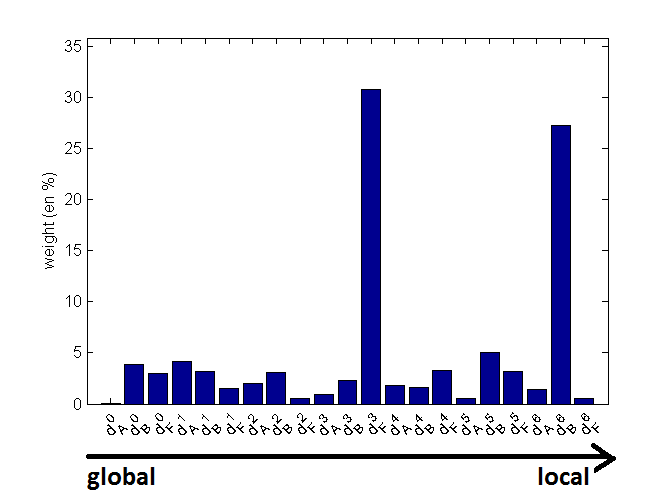
\includegraphics[width = 3in]{SonyAIBO_weight_V2}} \
	\subfloat[SonyAIBO]{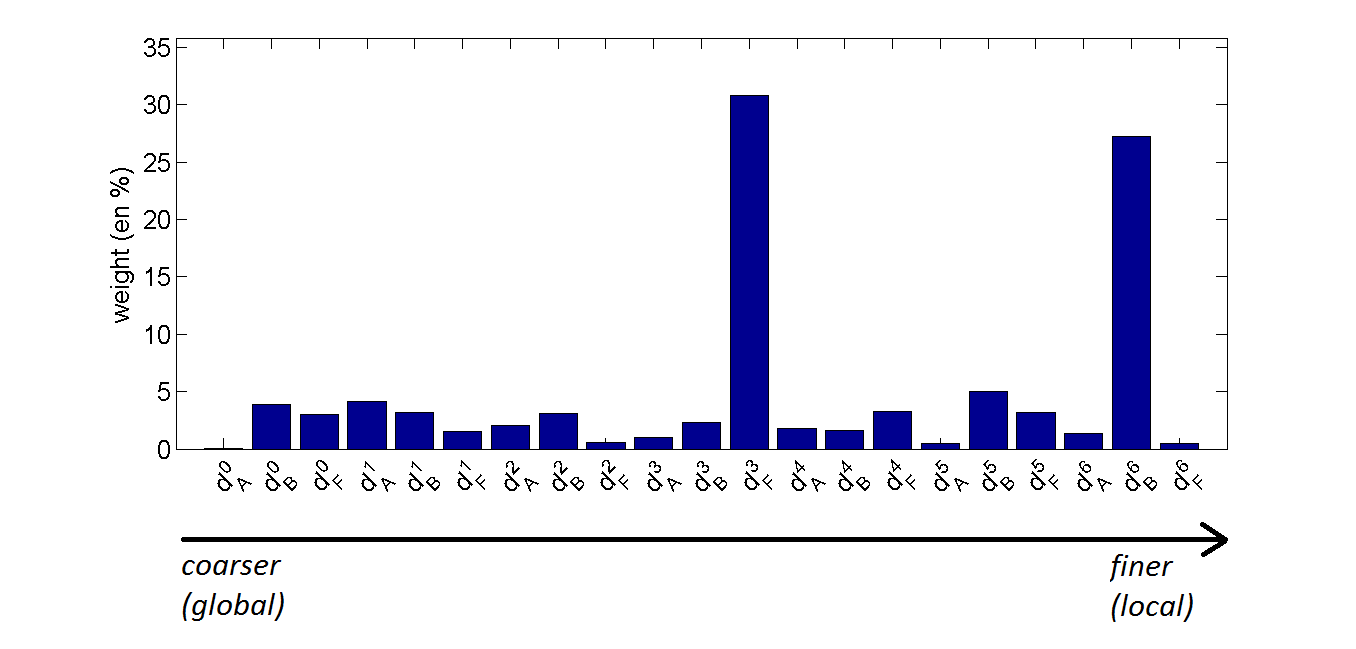
\includegraphics[width = 3.5in]{SonyAIBORobotSurface_NoDelay_bar2}} \
	\subfloat[Beef]{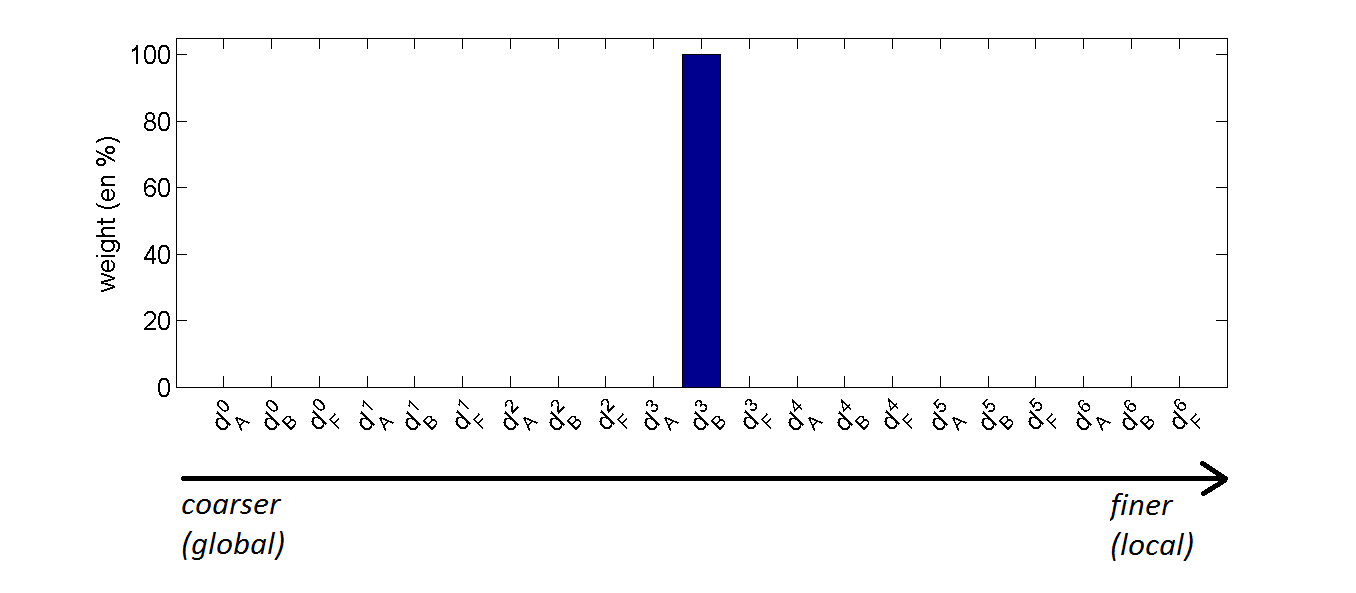
\includegraphics[width = 3.5in]{Beef_NoDelay_bar2}}\    
	\subfloat[CinC ECG torso]{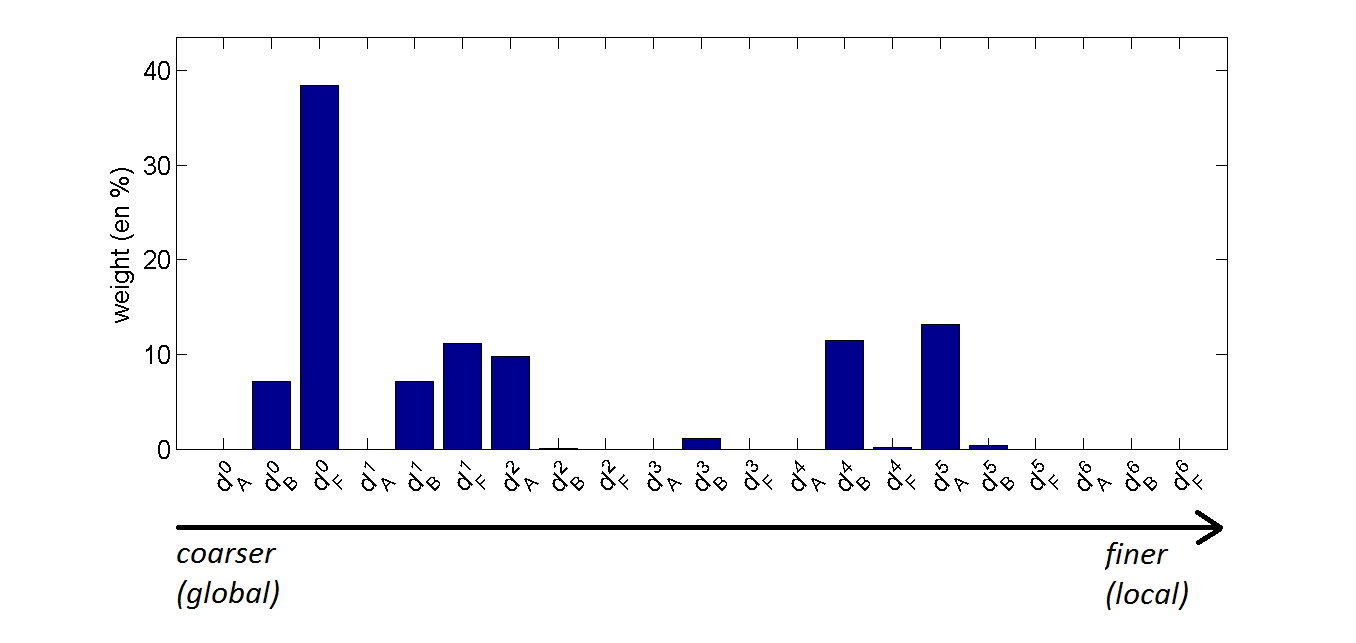
\includegraphics[width = 3.5in]{CinC_ECG_torso_NoDelay_bar2}} \
	\subfloat[FaceFour]{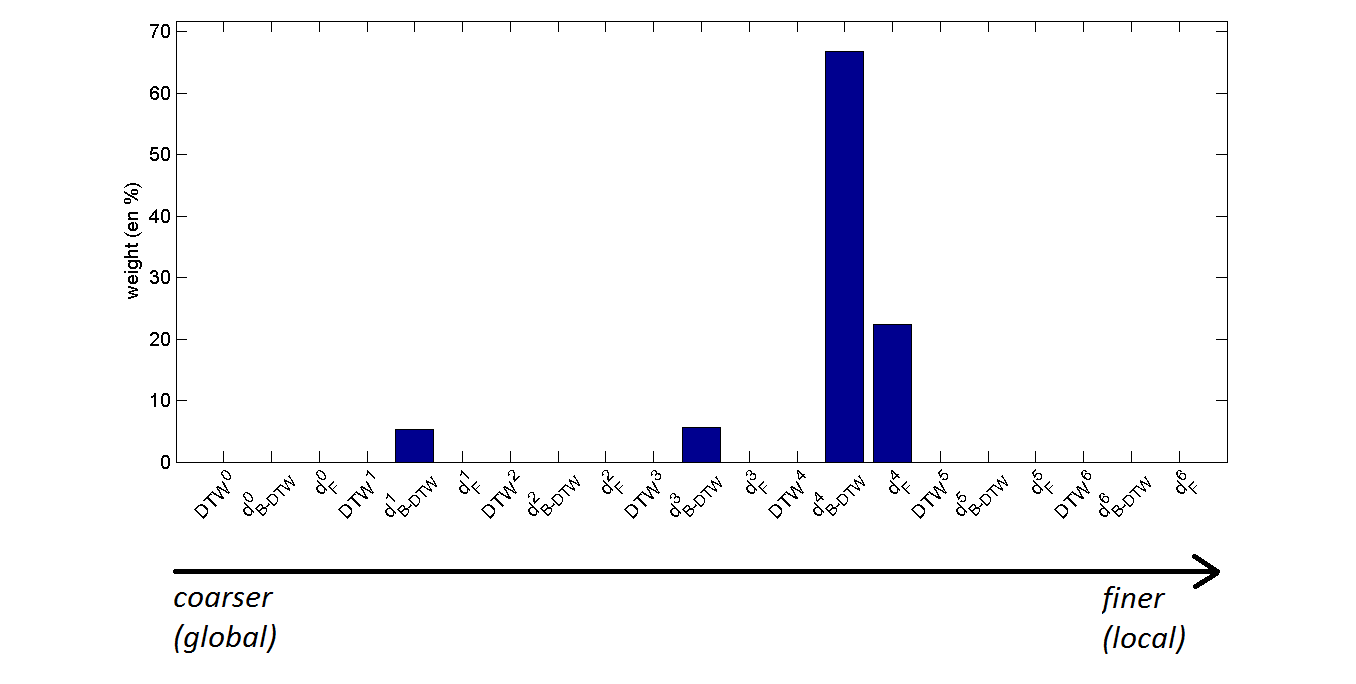
\includegraphics[width = 3.5in]{FaceFour_DTW_bar2}} 
	\caption{{\sc m}$^2${\sc tml} feature weights for 4 datasets.}
	\label{fig:w}
\end{figure}

\begin{figure}[h!]
	\centering
	\subfloat[SonyAIBO]{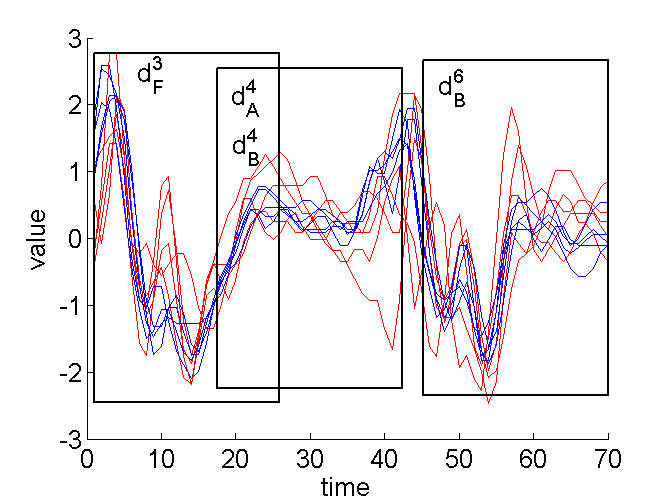
\includegraphics[width = 2.7in]{SonyAIBORobotSurface_NoDelay_TS}} 
	\subfloat[Beef]{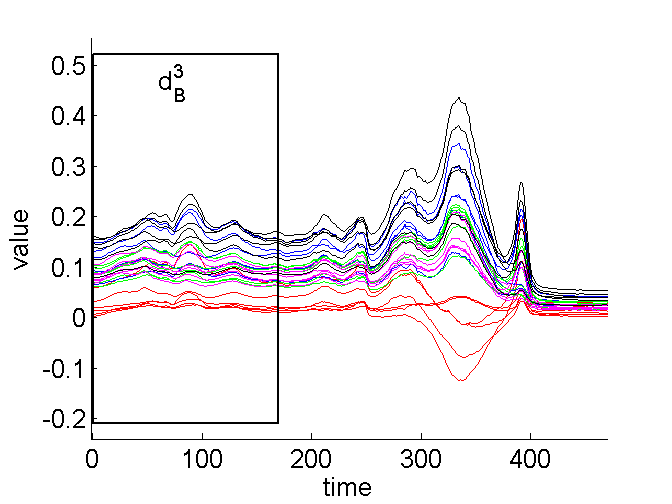
\includegraphics[width = 2.7in]{Beef_NoDelay_TS}} \   
	\subfloat[CinC ECG torso]{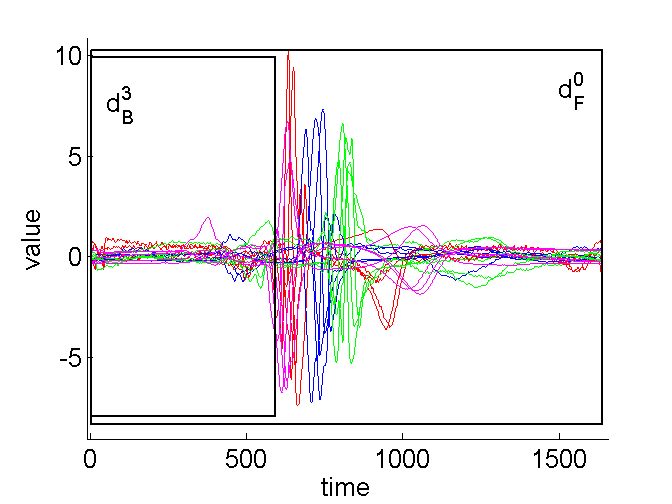
\includegraphics[width = 2.7in]{CinC_ECG_torso_NoDelay_TS}}
	\subfloat[FaceFour]{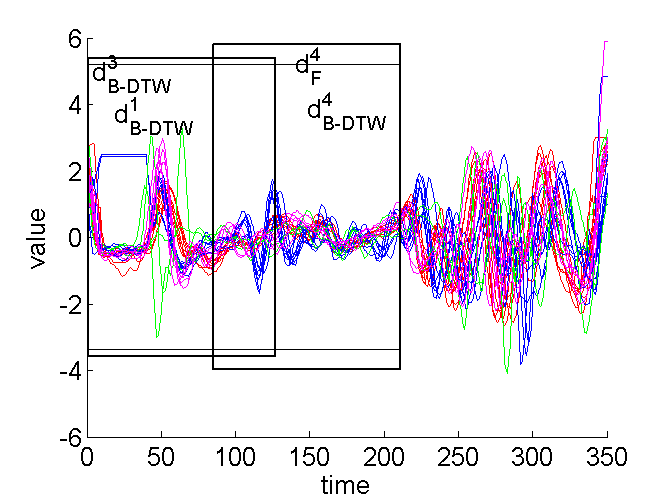
\includegraphics[width = 2.7in]{FaceFour_DTW_TS2}} 
	\caption{Temporal representation of the top {\sc m}$^2${\sc tml} feature weights for 4 datasets.}
	\label{fig:temporal_rep}
\end{figure}


%\begin{figure}[h!]
%	\centering
%	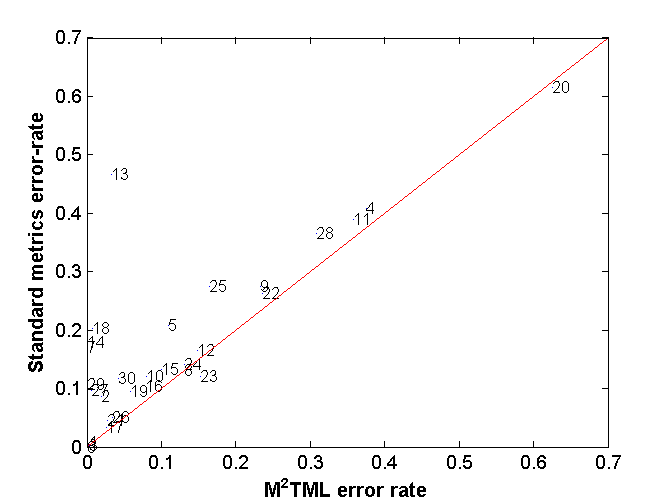
\includegraphics[width=0.6\linewidth]{images/Stand_m2tml}
%	\caption{Standard (Euclidean distance $d_A$  and {\sc dtw}) {\it vs.} {\sc m}$^2${\sc tml} ($D$ and $D_{\mathcal{H}}$) metrics }
%	\label{fig:error1}
%\end{figure}
%\begin{figure}[h!]
%	\centering
%	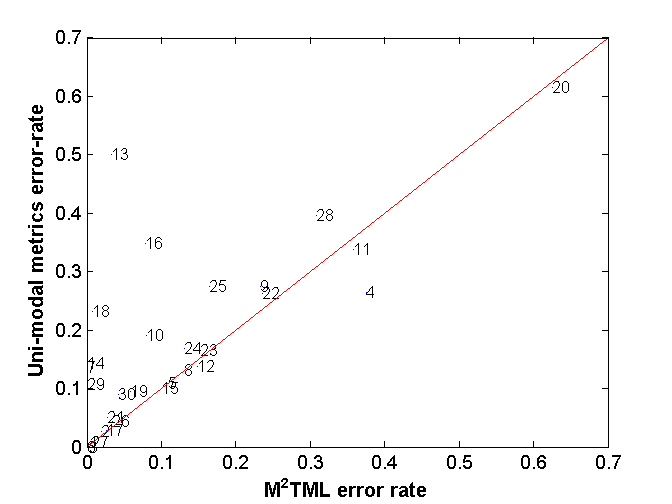
\includegraphics[width=0.6\linewidth]{images/Unimod_m2tml}
%	\caption{Best Uni-modal ({\sc dtw} and $d_{B-\mbox{\sc dtw}}$) {\it vs.} {\sc m}$^2${\sc tml} ($D$  and $D_{\mathcal{H}}$) metrics }
%	\label{fig:error2}
%\end{figure}

\begin{figure}[h!]
	\centering
	\subfloat[FaceFour ($d_{B-\mbox{\sc dtw}}$, stress: 20,1\%)]{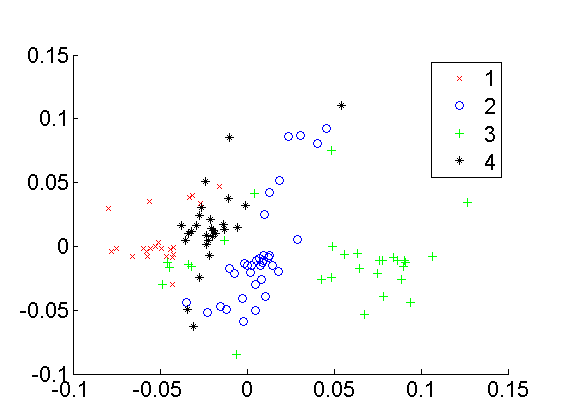
\includegraphics[width = 3in]{FaceFourALL_DTWDB_2}} 
	\subfloat[FaceFour ($D$, stress: 18,9\%)]{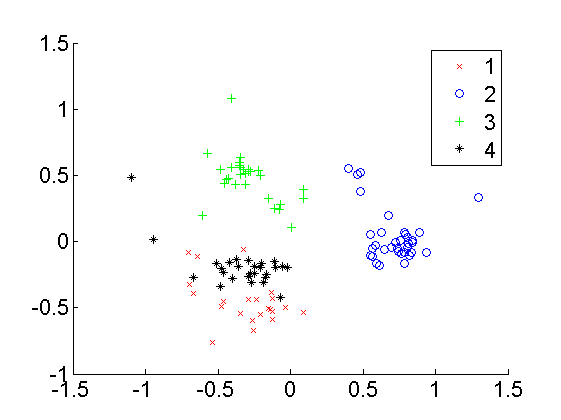
\includegraphics[width = 3in]{FaceFourALL_D_Delay_3}} \  
%	\subfloat[]{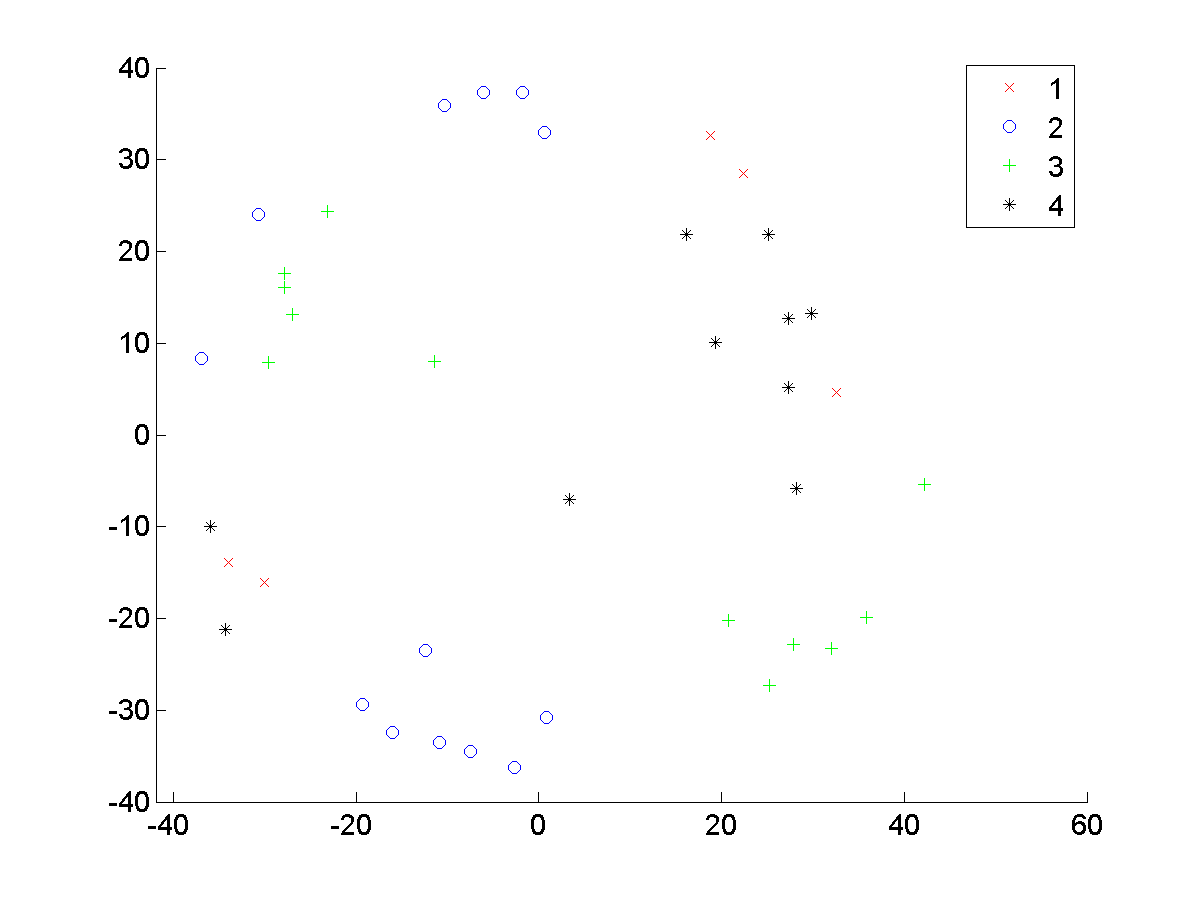
\includegraphics[width = 3in]{CinC_ECG_torso_MDS_DA}} 
%	\subfloat[]{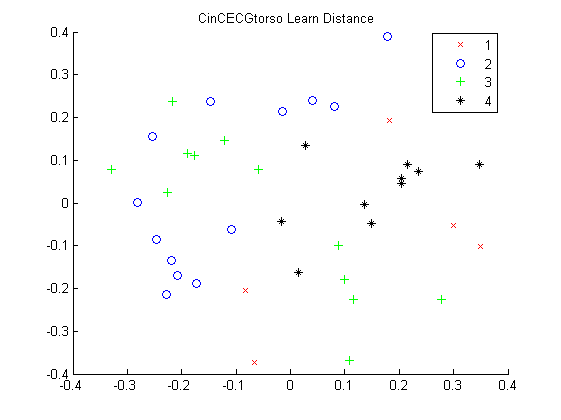
\includegraphics[width = 3in]{CinC_ECG_torso_MDS_After}}  
	\caption{{\sc mds} visualization of the $d_{B-\mbox{\sc dtw}}$ (Fig. a) and $D$ (Fig. b) dissimilarities for FaceFour}
	\label{fig:mds}
\end{figure}

\newpage
\subsection{Effect on the neighborhood before and after learning}
In the last part, we compare the global effect of the alternative and {\sc m}$^2${\sc tml} metrics  on the $1$-NN neighborhood distribution and class discrimination. For that, a MultiDimensional Scaling\footnote{Matlab function: mdscale for metrics and non metrics} ({\sc mds}) is used to visualize the distribution of samples according to their pairwise  dissimilarities. Briefly, we recall that {\sc mds} is a method of visualizing the proximity between samples in a dataset (Section \ref{sec:property_metric}). Given an input dissimilarity matrix, we can project the time series on a 2-dimensional plot whose configuration reproduces the best the dissimilarities between the time series. Note that the {\sc mds} representation has no link with the dissimilarity space representation whose dimensions are basic temporal metrics.

For FaceFour, Fig. \ref{fig:mds} shows the first obtained plans and their corresponding stresses, the classes being indicated in different symbols and colors. We can see distinctly the effect of the learned  $D$ that leads to  more compact and more isolated classes with  robust  neighborhoods for 1-NN classification ({\it i.e.}, closer pull pairs and far away push pairs) than  the best alternative metric $d_{B-\mbox{\sc dtw}}$ that shows more overlapping classes and heterogeneous neighborhoods.
%\begin{figure}[h!]
%	\centering
%	% 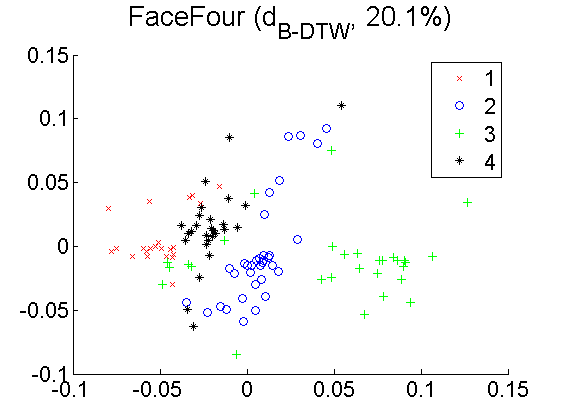
\includegraphics[width=0.6\linewidth]{images/FaceFourALL_DTWDB_1} \hspace{-0.45cm}
%	% 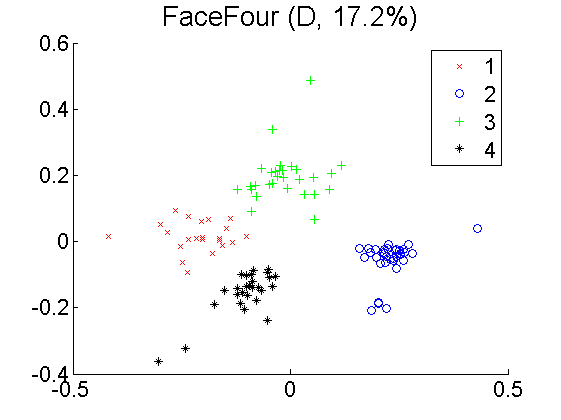
\includegraphics[width=0.6\linewidth]{images/FaceFourALL_D_Delay_1}
%	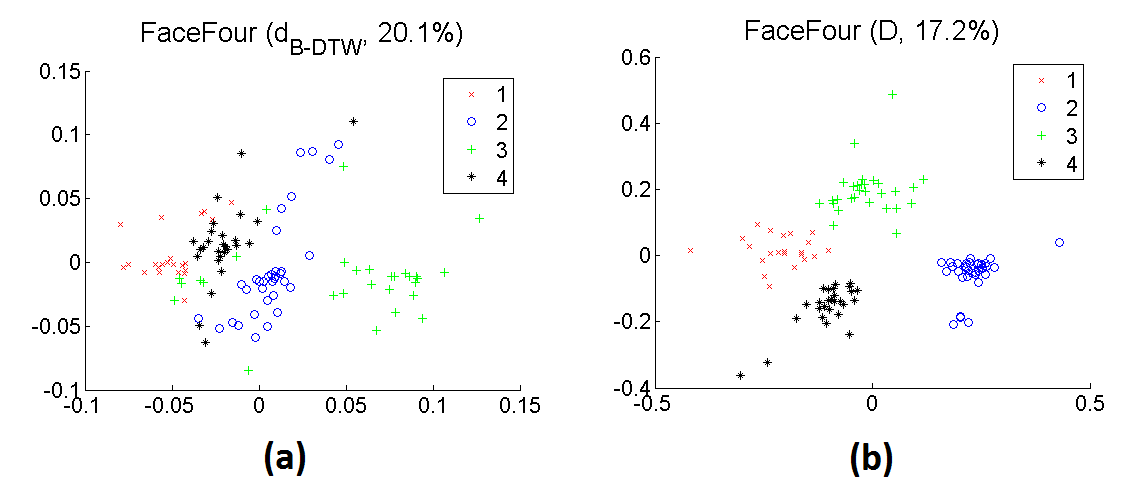
\includegraphics[width=1\linewidth]{FaceFour}
%	\caption{{\sc mds} visualization of the $d_{B-\mbox{\sc dtw}}$ (left) and $D$ (right) dissimilarities for FaceFour data}
%	\label{fig:mds}
%\end{figure} 

\section{Conclusion of the chapter}
%%% Local Variables: 
%%% mode: latex
%%% TeX-master: "../roque-phdthesis"
%%% End: 
% This paper proposes a new Multi-modal and Multi-scale Temporal Metric Learning ({\sc m}$^2${\sc tml}) framework  for large margin time series nearest neighbors classification. 
% For this, time series are embedded  into a  dissimilarity space  where a  function combining several modalities at different temporal scales can be learned,  driven jointly by a pairwise {\sc svm} and nearest neighbors metric learning framework.  Thanks to the 'kernel trick',  the {\sc m}$^2${\sc tml} approach  provides a temporal metric learning solution for linear as well as  non linear contexts. A sparse and interpretable variant of the solution  shows the ability of the learned temporal metric to localize accurately discriminative  modalities as well as their temporal scales.   
The large conducted experiments and the impressive performances obtained  attest the efficiency of the learned {\sc m}$^2${\sc tml} metrics for time series nearest neighbors classification. As discussed, the datasets encompass time series that involve global or local temporal comparison, require or not time warping, with linearly or non linearly separable neighborhoods. \\
Finally, let us underline the merit of the {\sc m}$^2${\sc tml}  solution, that not only leads to equivalent or better performances from the standard metrics (Euclidean distance, Dynamic time warping), but also provides a comprehensive and fine-grained information about  which modalities are mostly discriminant, how they should be combined and precisely at which temporal granularity (localization). 